\chapter{Particle Physics for Data Scientists}



\section{The Preliminaries}


\subsection{Problems with the standard model}

What makes us unhappy?
\begin{itemize}
  \item Matter and Antimatter inequivalence.
  \item 19 Arbitrary constants.
  \item Why is Gravity so weak.
\end{itemize}


\subsection{The Particles we want to detect}

\begin{figure}[H]
  \centering
  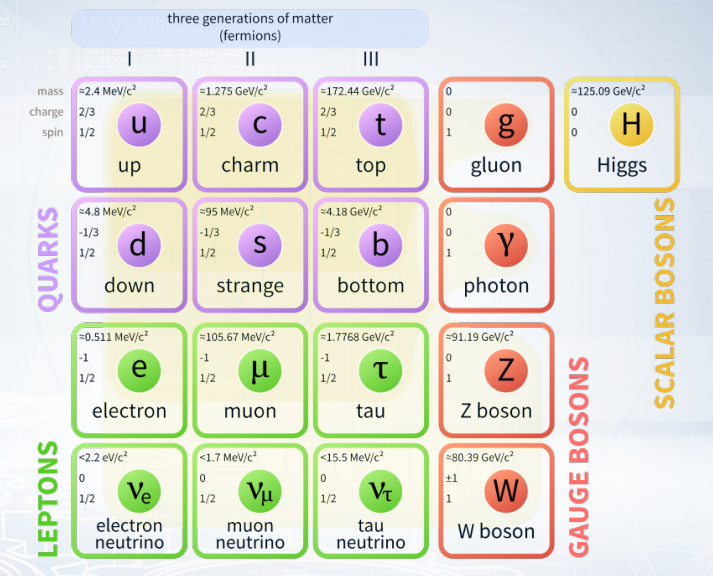
\includegraphics[width=0.4\linewidth]{img/hadron/particleid-list.png}
  \caption{List of Particles of different types}
  \label{fig:particleid-list}
\end{figure}

The following are types of particles we want to defect.
\begin{multicols}{3}
  \begin{itemize}
    \item muon
    \item kon
    \item pion
    \item proton
    \item electron
  \end{itemize}
\end{multicols}



\subsection{The Experiments in LHC}

There are 4 major detectors
\begin{itemize}
  \item ALICE (A Large Ion Collider Experiment) is a heavy-ion detector on the Large Hadron Collider (LHC) ring. It is designed to study the physics of strongly interacting matter at extreme energy densities, where a phase of matter called quark-gluon plasma forms.
  \item ATLAS (A Toroidal LHC ApparatuS) is one of two general-purpose detectors at the Large Hadron Collider (LHC). It investigates a wide range of physics, from the search for the Higgs boson to extra dimensions and particles that could make up dark matter. Although it has the same scientific goals as the CMS experiment, it uses different technical solutions and a different magnet-system design. It has a cylindrical structure and measures particles in all directions.
  \item CMS (Compact Muon Solenoid) is a general-purpose detector at the Large Hadron Collider (LHC). It has a broad physics programme ranging from studying the Standard Model (including the Higgs boson) to searching for extra dimensions and particles that could make up dark matter. Although it has the same scientific goals as the ATLAS experiment, it uses different technical solutions and a different magnet-system design.
  \item LHCb (Large Hadron Collider Beauty) experiment specializes in investigating the slight differences between matter and antimatter by studying a type of particle called the "beauty quark", or "b quark". It is a single arm forward spectrometer.
\end{itemize}

We smash bunches of protons ('events'), record the pixels ('hits'), reconstruct trajectories ('jets', 'showers', 'tracks'), and we perform Statistical analysis on them.

A Trigger System is a system that uses criteria to rapidly decide which events in a particle detector to keep when only a small fraction of the total can be recorded.


\subsection{Simulation Package}

\begin{itemize}
  \item http://www.genie-mc.org/
  \item http://home.thep.lu.se/Pythia/: Nutrino Simulations
  \item GEANT4: http://geant4.web.cern.ch/: Particles interacting with matter.
  \item FLUKA: http://www.fluka.org/fluka.php
\end{itemize}


\subsection{Feynman Diagrams}

\begin{figure}[H]
  \centering
  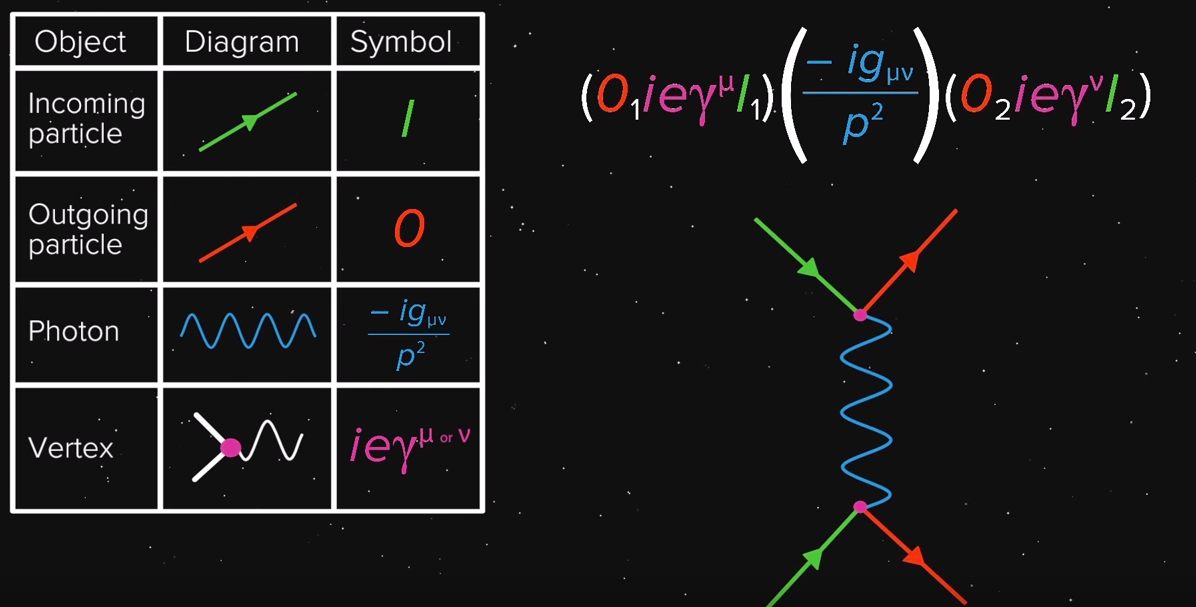
\includegraphics[width=0.8\linewidth]{img/hadron/preliminary-feynman-diagram.png}
  \caption{A Sample Feynman Diagram for scattering of Two electron by the transfer of one Photon}
  \label{fig:preliminary-feynman-diagram}
\end{figure}



\section{The Large Hadron Collider Setup}

\begin{figure}[H]
  \centering
  \begin{subfigure}[b]{0.5\textwidth}
    \centering
    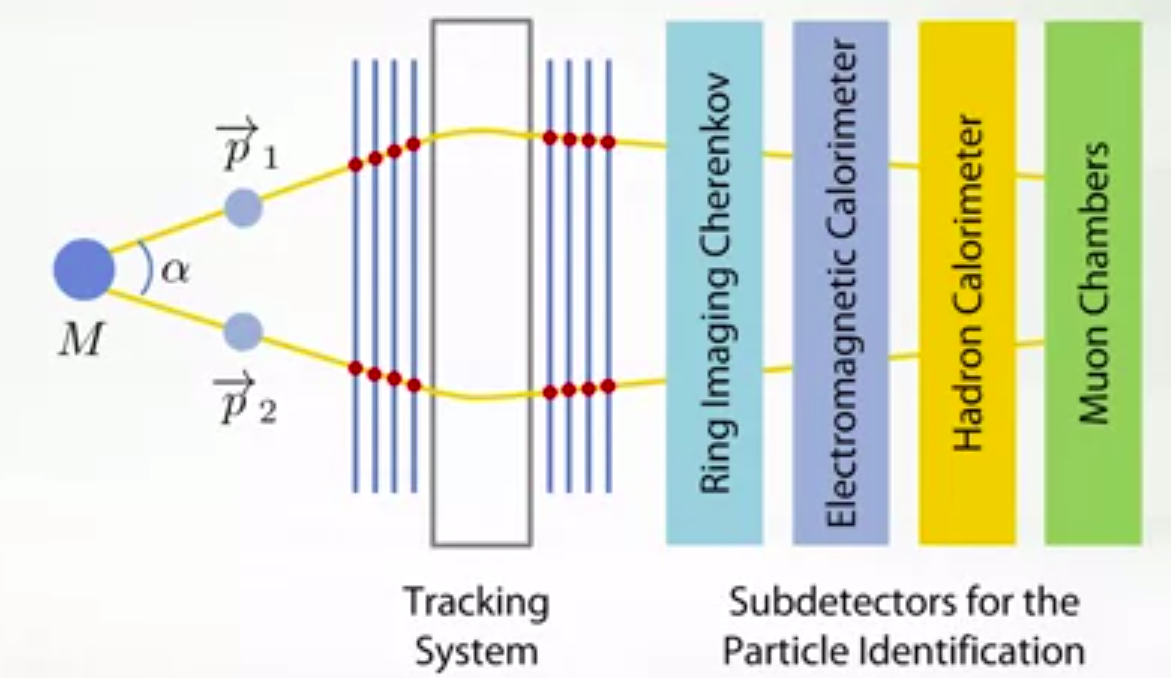
\includegraphics[width=\linewidth]{img/hadron/particleid-detector-setup.png}
    \caption{Detector Setup of the LHC}
    \label{fig:particleid-detector-setup}
  \end{subfigure}
  \begin{subfigure}[b]{0.4\textwidth}
    \centering
    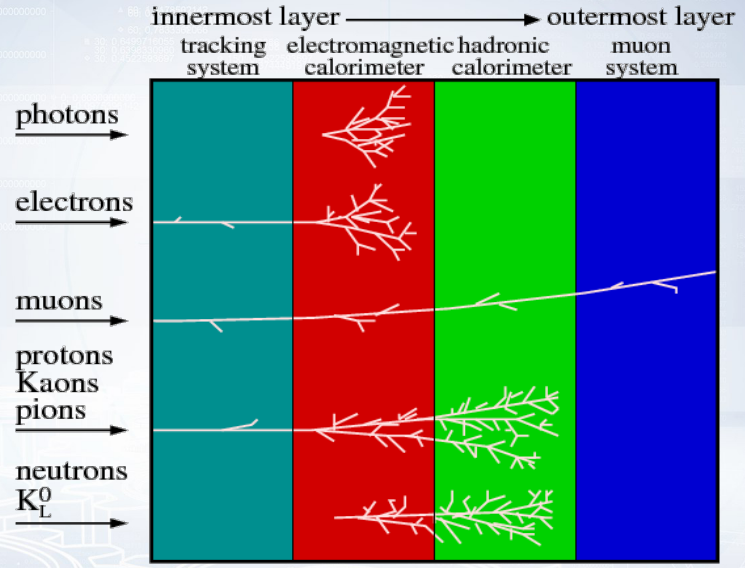
\includegraphics[width=\linewidth]{img/hadron/particleid-tracking.png}
    \caption{The tracks made in the Chambers}
    \label{fig:particleid-tracking}
  \end{subfigure}
\end{figure}


\subsection{Tracking System}

The first system of detectors, stands before particle collision area. Important for parameter estimation. 

There are several layers of sensors that measure hits, and allow us to recognise particle trajectories.
There is also a Magnetic Field that allows us to measure momentum (using radius of curvature in the field).

We have the following conservation equationsm wgeb a particle $D^0$ with mass $m$ breaks into a $K^-$ with mass $m_1$ and a $\pi^+$ with mass $m_2$, and they go away from each other at angle $\alpha$:
\begin{eqnarray}
  E_m &=& E_1 + E_2 \\
  \hat{p_m} &=& \hat{p_1} + \hat{p_2} \\
  E^2 &=& p^2 c^2 + m^2 c^4 \\
  M^2 &=& m_1^2 + m_2^2 + \frac{2}{c^4} (E_1 E_2 - p_1 p_2 c^2 cos\alpha)
\end{eqnarray}

\subsubsection{Problem: Track Pattern Recognition} Recognizing hits that belong to the same track. Currently we have the following methods.
\begin{itemize}
  \item Half Transform and Kalman Filtering. (Statistical, computationally cheaper.)
  \item Hopfield Neural Netorks. (Denby Peterson and Cellular Automaton.)
  \item Convolutional Nerual Networks (classify result as correct or wrong). Recurrent Neural Netorks (predict the next hit location).
\end{itemize}
We can then combine these particle tracks into decays.

\subsection{Ring Imaging Chernekov Detector (RICH)}

This is the first detector because it does not affect the flight of the particle.

\begin{figure}[H]
  \centering
  \begin{subfigure}[b]{0.45\textwidth}
      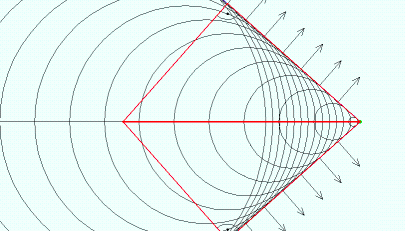
\includegraphics[width=\linewidth]{img/hadron/particleid-chernekov-wavefronts.png}
      \caption{Chernekov Simulation}
  \end{subfigure}
  \begin{subfigure}[b]{0.30\textwidth}
      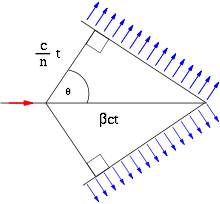
\includegraphics[width=\linewidth]{img/hadron/particleid-cherenkov-angles.png}
      \caption{Chernekov Angles}
  \end{subfigure}
  \begin{subfigure}[b]{0.45\textwidth}
    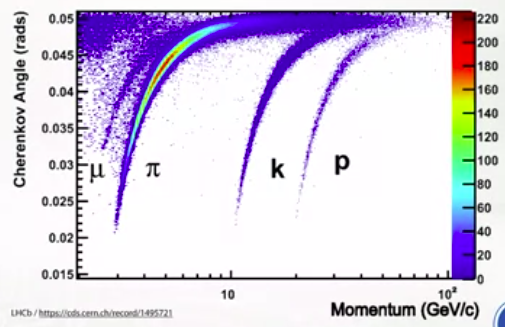
\includegraphics[width=\linewidth]{img/hadron/particleid-chernekov-graph.png}
    \caption{Chernekov Radiation Graphs}
  \end{subfigure}
  \label{fig:particleid-chernekov-wavefronts}
  \caption{Registers in Processor Design}
\end{figure}

Here is the angle of the Chernokov radiation, derivable using simple geometric means and some special relativity in terms of the momentum.
\begin{equation}
  p = \frac{mc\beta}{\sqrt{1 - v^2/c^2}}
\end{equation}
\begin{equation}
  cos \theta = \frac{1}{n\beta} = \frac{\sqrt{p^2 + m^2c^2}}{np}
\end{equation}
From the figure above, and the equation for it's analytical feel, that we can figure out the mass of the particle and thereby which particle it is.

% ISSUE: 5:40 Kaon and Pion rings.

\subsection{Calorimeter - Electromagnetic and Hadronic}

Electromagnetic stops all but than muons and quarks. Hadron calorimeter stops the quarks.

\begin{equation}
  E_C = E_0 e^{\frac{x}{X_0}}
\end{equation}
\begin{equation}
  X_{max} = X_0 ln(\frac{E_0}{E_c})
\end{equation}
\begin{equation}
  N = E_0 / E_c
\end{equation}

After this we have crystals and scintillation counters, that measure the count and energy of particles, The electrons and photons, and since we measure energy, we already have momenta from the tracking system., this gives us the Mass, so we can identify them.

\subsection{Muon Chambers}

Muons do not interact well with matter. So we have multiple layers of metal to slow down the muons, they activate the chambers, we will extrapolate the data to get which particles in the tracking system were muons. We can also get the energy from how far they go in the muon chambers.


\subsection{How to make a classifier uniform}

\subsubsection{The problem}
\begin{eqnarray}
1 - false\;positive\;rate &=& background\;rejection \\
true\;positive\;rate &=& signal\;efficiency
\end{eqnarray}
We want to have no dependence of the ROC AUC on all the momenta.

\begin{eqnarray}
  L_{ada} &=& \Sigma e^{-\gamma_i S_i} \\
  L_{flat} &=& \Sigma_b w_b \int |F_b(s) - F(s)|^2 ds \\
  L_{adaflat} &=& L_{ada} + \alpha L_{flat}
\end{eqnarray}
This is imposing an additional loss over the ADA boost function to make it less dependent on the momentum, alpha is a parameter we can tune to weight flatness over fit quality.

\subsection{Adversarial Neural Networks}

Minimizing dependencies on Mass, Momentum, etc. can also be done using adversarial neural networks. One network performs classification, and feeds it's output to the other which tries to guess the momentum/mass from the output, if it can do this well, the model is bad, i.e. not flat. So, our new loss is $Loss_{classification} + f(Loss_{adversarial})$.


\section {Discovering New Physics}

% TODO: Learn about different classes of Particles in Standard model, SUSY Particles
% Particle-Data-Group has breaking of all particles

\subsection{NoEther's theorem}

NoEther's theorem claims that the conservation laws we have are based on certain symetries.
Here is a list of some of them.
\begin{itemize}
  \item Time Inversion: Energy
  \item Space Translation: Linear momentum
  \item Space Rotation: Angular momentum
  \item Charge Conjugation and Parity: Time Isotropy
  \item Charge, Lepton Number: Gauge Symetries 
\end{itemize}

\subsection{}

CvM test 
\begin{equation}
  CvM = \Sigma_{region} \int |F_{region}(s) - F_{global}(s)|^2 dF_{global}(S)
\end{equation}

% UBoost BDT

\subsection{Doping}

